\documentclass[12 pt, letterpaper]{exam}
\printanswers
\usepackage{amsfonts}
\usepackage{graphicx}
\usepackage{amsthm}
\usepackage{amssymb}
\usepackage{amsmath}
\usepackage{enumerate, mathrsfs}
\usepackage[framed,indented,numbered,autolinebreaks,useliterate]{mcode}


\theoremstyle{definition}
\newtheorem{ex}{Example}
\newtheorem{df}{Definition}
\newtheorem{thm}{Theorem}
\newtheorem{prob}{Problem}

\newcommand{\suchthat}{\,\Big{|}\,}
\newcommand{\ZZ}{\mathbb{Z}}
\newcommand{\QQ}{\mathbb{Q}}
\newcommand{\NN}{\mathbb{N}}
\newcommand{\RR}{\mathbb{R}}
\newcommand{\CC}{\mathbb{C}}
\newcommand{\dd}{\,\,\textrm{d}}

\firstpageheader{Math 3900 Spring 2019}{Homework 1}{Instructor:  J. Haga}
\begin{document}
\noindent Due:  Friday January 18 by 11:59PM.  The first two problems of this homework set depend heavily on the following example.
\ex In this example we use MATLAB to determine the value(s) of $c$ guaranteed by the Mean Value Theorem for the function $f(x) = x^3-x$ on the interval $[-1.5,1.2]$.  In this example, $f$ is a cubic, and since $f'$ is quadratic, we can solve this problem exactly using calculus and algebra:
\begin{align*}
&f(x) = x^3-x\\
&f(1.2)=0.528,\quad f(-1.5)=-1.875\quad \rightarrow  \quad \frac{f(1.2)-f(-1.5)}{1.2-(-1.5)} = 0.89\\
\\
&f'(x) = 3x^2-1\\
&f'(c) = 3c^2-1=0.89 \quad \quad \rightarrow \quad \quad c = 0.7937,\,\,-0.7937
\end{align*}

\noindent For more general functions over more general intervals it may not be easy or possible to analytically determine [even approximations of] the desired value of $c$.  We will therefore utilize MATLAB to find approximate values of $c$, via a method which can be applied to a wide variety of functions on a wide variety of intervals.
\vskip 2ex
\noindent We begin by defining symbolic variable $x$, and the symbolic variable $f$ defined in terms of $x$:
\lstset{numbers=left}

\begin{lstlisting}
>> syms f(x)
>> f(x) = x^3-x

f(x) =

x^3 - x
\end{lstlisting}
\vskip 2ex
\noindent We have MATLAB determine the derivative of $f$:
\lstset{numbers=left,firstnumber=last}
\begin{lstlisting}
>> df(x)=diff(f,x)

df(x) =

3*x^2 - 1
\end{lstlisting}
\vskip 2ex

\noindent MATLAB can automatically determine the desired value(s) of $c$:

\begin{lstlisting}
>> A=solve(df(x)==(f(1.2)-f(-1.5))/(1.2-(-1.5)))

A =

 -(3*7^(1/2))/10
  (3*7^(1/2))/10
\end{lstlisting}
\vskip 2ex
\noindent We desire decimal approximations of $c$ rather than algebraic expressions:

\begin{lstlisting}
>> double(A)

ans =

   -0.7937
    0.7937
\end{lstlisting}
\vskip 2ex
\noindent From this we see that we have arrived at the same values of $c$ we obtained analytically.  We may thus use MATLAB to determine the equations of the lines tangent to $f$ at each of the values of $c$ given:

\begin{lstlisting}
>> df(A)

ans =

 89/100
 89/100

>> f(A)

ans =

  (111*7^(1/2))/1000
 -(111*7^(1/2))/1000
\end{lstlisting}

\vskip 2ex

\noindent Again, we prefer decimal approximations:

\begin{lstlisting}
>> double(df(A))

ans =

    0.8900
    0.8900

>> double(f(A))

ans =

    0.2937
   -0.2937
\end{lstlisting}
\vskip 2ex

\noindent From this we can determine the equations of the two tangent lines:
\begin{align*}
t_1(x)&= 0.89(x+0.7937)+0.2937\\
t_2(x)&= 0.89(x-0.7937)-0.2937,
\end{align*}
\noindent as well as the equation of the line segment connecting both ends of our graph:  $$M(x) = \left(\frac{f(1.2)-f(-1.5)}{(1.2-(-1.5))}\right)(x-1.2)+f(1.2),$$ and we can command MATLAB to graph these on the same axes:

\begin{lstlisting}
>> M(x)=(f(1.2)-f(-1.5))/(1.2-(-1.5))*(x-1.2)+f(1.2)

M(x) =

(89*x)/100 - 27/50

>> B=[f;M;df(A).*([x;x]-A)+f(A)]

B(x) =

                        x^3 - x
             (89*x)/100 - 27/50
 (89*x)/100 + (189*7^(1/2))/500
 (89*x)/100 - (189*7^(1/2))/500

>> fplot(B,[-1.5,1.2])
\end{lstlisting}
\vskip 2ex
We obtain the following output:
\begin{center}
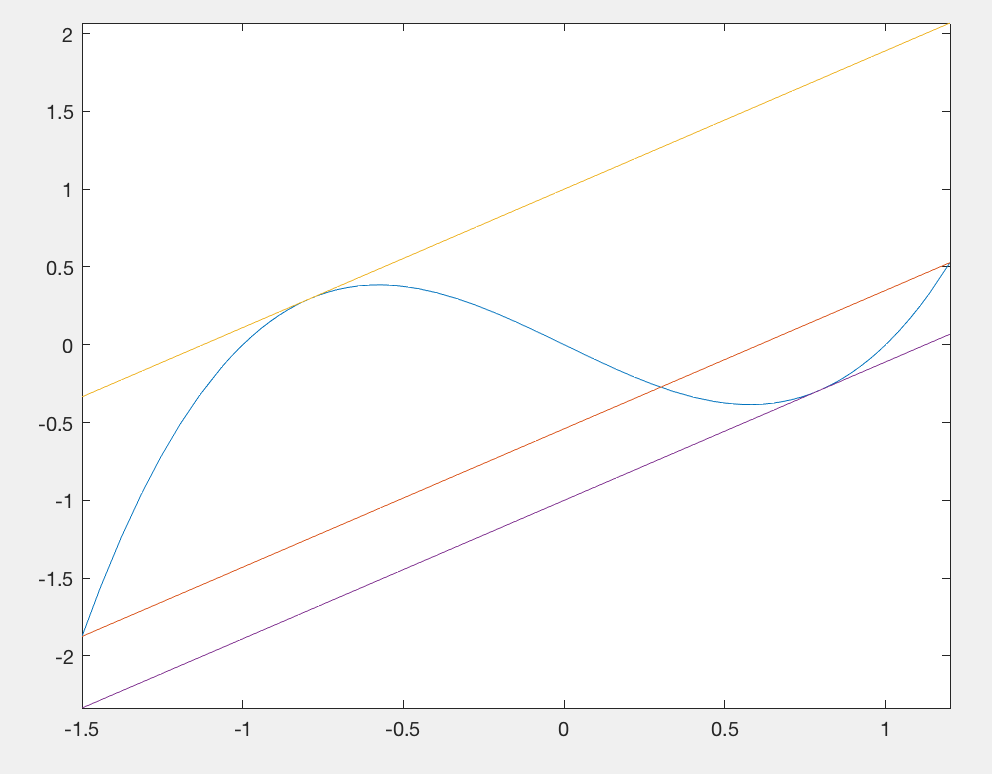
\includegraphics[width=3in]{hw01img01}
\end{center}

\newpage
\begin{questions}
\question
\begin{parts}
\part[5] What is the advantage of the command
\lstset{numbers=none}
\begin{lstlisting}
>> A=solve(df(x)==(f(1.2)-f(-1.5))/(1.2-(-1.5)))
\end{lstlisting}
\noindent versus the possibility
\begin{lstlisting}
>> solve(df(x)==(f(1.2)-f(-1.5))/(1.2-(-1.5)))
\end{lstlisting}
\noindent in line 12 of the command window shown above?

\begin{solution}
The top command stores the solution in variable A, which allows you to do operations with the solution afterwards.
\end{solution}

\part[5] Why do we use {\tt df(A).*([x;x]-A)} versus {\tt df(A)*([x;x]-A)} (i.e. without the period before the multiplication) in line 56 of the command window above?

\begin{solution}
We use {\tt df(A).*([x;x]-A)} because it does multiplication on each element of the matrix {\tt df(A)} whereas using just {\tt *} does matrix multiplication.
\end{solution}

\end{parts}

\question Utilize commands similar to the ones given above to:
\begin{parts}
\part[10] determine the value(s) of $c$ guaranteed by the Mean Value Theorem for the function $\displaystyle{f(x)=\frac{x(x-1)(x-2)(x-3)(x-4)}{2}}$ on the interval $[0.2,3.7]$,
\begin{solution}

   \noindent Here we set the function and derive.
   \begin{lstlisting}
>> syms x
>>
>> f(x)=(x*(x-1)*(x-2)*(x-3)*(x-4))/2

f(x) =

   (x*(x - 1)*(x - 2)*(x - 3)*(x - 4))/2

>> df(x)=diff(f,x)

df(x) =

   (x*(x - 1)*(x - 2)*(x - 3))/2 + (x*(x - 1)*(x - 2)*(x - 4))/2 + (x*(x - 1)*(x - 3)*(x - 4))/2 + (x*(x - 2)*(x - 3)*(x - 4))/2 + ((x - 1)*(x - 2)*(x - 3)*(x - 4))/2
   \end{lstlisting}
   \newpage\noindent Here we solve using {\tt df(x)} and the threshold values, thus finding the values of $c$ guaranteed by the Mean Value Theorem.
   \begin{lstlisting}
>> A=solve(df(x)==(f(.2)-f(3.7))/(.2-(3.7)))

A =

   2 - (6 - 10711^(1/2)/25)^(1/2)/2
   (6 - 10711^(1/2)/25)^(1/2)/2 + 2
   2 - (10711^(1/2)/25 + 6)^(1/2)/2
   (10711^(1/2)/25 + 6)^(1/2)/2 + 2

>> double(A)

ans =

   1.3180
   2.6820
   0.4079
   3.5921
   \end{lstlisting}
\end{solution}
\part[10] determine the equation of the line segment $M(x)$ connecting the endpoints of the graph described in part (a),
\begin{solution}
   We use point slope form to determine the equation of the line $M(x)$ between the two points.
   \begin{lstlisting}
>> M(x) = ((f(3.7)-f(0.2))/(3.7-(0.2))) * (x - 3.7) + f(3.7)

M(x) =

   172161/100000 - (3789*x)/4000
   \end{lstlisting}
   The MATLAB calculation gives us the line (to 4 decimal places):
   \begin{align*}
   M(x)&= -0.9473x+1.7216
   \end{align*}
\end{solution}
\newpage
\part[10] determine the equations of the tangent lines at each of the values of $c$ determined in part (a) (there are 4 of them for this function on this interval), and
\begin{solution}
   We used MATLAB to calculate out our tangent lines $T(x)$ (solutions cut for brevity):
   \begin{lstlisting}
>> T(x) = (df(A) .* ([x;x;x;x] - A)) + f(A)

T(x) =
  (x + (6 - 10711^(1/2)/25)^(1/2)/2 - 2)* ...
  ((6 - 10711^(1/2)/25)^(1/2)* ...
  (x + (10711^(1/2)/25 + 6)^(1/2)/2 - 2)* ...
  ((10711^(1/2)/25 + 6)^(1/2)* ...
   \end{lstlisting}
   Cleaned up, our tangent line functions look like:
   $$T_1(x) = -0.9473x + 0.6037$$
   $$T_2(x) = -0.9473x + 3.1853$$
   $$T_3(x) = -0.9473x + 2.1765$$
   $$T_4(x) = -0.9473x + 1.6125$$
\end{solution}
\newpage
\part[10] plot $f$, $M$, $t_1$, $t_2$, $t_3$, and $t_4$ on the same axes (in MATLAB).
\begin{solution}
   We then concatenated all of our functions into one array and plotted that array on our bounds:
   \begin{lstlisting}
>> B=[f;M;T];
>> fplot(B, [0.2,3.7]);
   \end{lstlisting}
   \begin{center}
      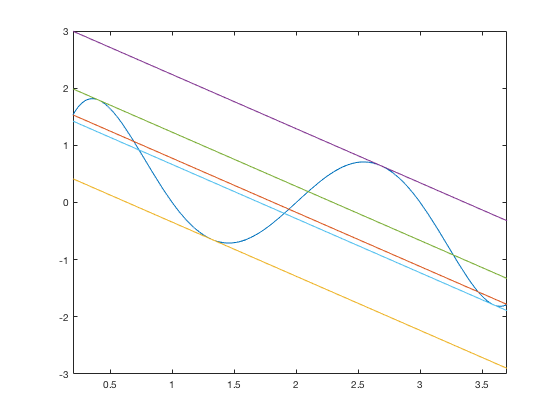
\includegraphics[width=3in]{plot-2d}
   \end{center}
\end{solution}
\end{parts}
Be sure to format your responses in a manner similar to the example above.  Include [a cleaned up version of] your command window, and the image of the plotted functions in your submission.

\newpage
\question[20] Use a Taylor polynomial to approximate $\cos(42^\circ)$ accurate to within $10^{-6}$.  Note:  the approximation is worth 5 points.  The remaining points are earned by demonstrating that you appropriately utilized the remainder formula $$R_n(x) = \frac{f^{(n+1)}(\xi(x))}{(n+1)!}(x-x_0)^{n+1}$$ to decide which Taylor polynomial $P_n(x)$ will approximate the desired value to within the given tolerance.  Make sure to compare your approximation to the approximation given by the Calculator application on your computer.
\begin{solution}
   We decided to do all of our calculations in radians, which means that instead of $42^\circ$, we are using $\frac{7\pi}{30}$. We chose an expansion point ($x_0$) of $\frac{\pi}{4}$ because it is a known value for both $\cos$ and $\sin$ and it is very close to the value we are trying to approximate. We started out trying to bound our remainder function, $$R_n(x) = \frac{f^{(n+1)}(\xi(x))}{(n+1)!}(x-x_0)^{n+1}.$$
   Because $f^{(n+1)}(x)$ will always be $sin(x)$, $cos(x)$, $-sin(x)$, or $-cos(x)$, we know that the max value of any of those functions for $\xi(x)$ will be $cos(42^\circ)$. We know this because $cos(x)$ starts at 1 and decreases, whereas $sin(x)$ starts at 0 and increases, and $cos(x) = sin(x)$ at $x = \frac{\pi}{4}$. Therefore, any value of $x$ less than $42^\circ$ for $cos(x)$ will bind the numerator, $f^{(n+1)}(\xi(x))$, of $R_n(x)$. We chose $\frac{\pi}{6}$, as it has a known value of $\frac{\sqrt{3}}{2}$ for $cos(x)$.
   
   Plugging in $x$ and $x_0$ with our bound, we get $$R_n(x) = \frac{\sqrt{3}/2}{(n+1)!}(-\frac{\pi}{4} - \frac{7\pi}{30})^{n+1}.$$

   Using this remainder function, we were able to show that we need $T_3$, as $R_3$ is equal to
   $2.7 * 10^{-7}$, which would make $T_3$ within $10^{-6}$.

  \begin{center}
   \begin{tabular}{||c c c c||}
   \hline
   \textbf{n} & \textbf{$T_n(x)$} & \textbf{$T_n(\frac{7\pi}{30})$} & \textbf{$R_n(x)$} \\
   \hline\hline
   0 & $\cos(\frac{\pi}{4})$ & 0.7071067812 & .04534 \\
   \hline
   1 & $\cos(\frac{\pi}{4}) - \sin(\frac{\pi}{4})(x-\frac{\pi}{4})$ & 0.7441308057 & .00119 \\
   \hline
   2 & $\cos(\frac{\pi}{4}) - \sin(\frac{\pi}{4})(x-\frac{\pi}{4}) - \frac{cos(\frac{\pi}{4})(x-\frac{\pi}{4})^2}{2}$ & 0.743161519 &  $2.1 * 10^{-5}$\\
   \hline
   3 & $\cos(\frac{\pi}{4}) - \sin(\frac{\pi}{4})(x-\frac{\pi}{4}) - \frac{cos(\frac{\pi}{4})(x-\frac{\pi}{4})^2}{2} + \frac{sin(\frac{\pi}{4})(x-\frac{\pi}{4})^3}{6}$ & 0.7431446017 & $2.7 * 10^{-7}$ \\
   \hline
  \end{tabular}
  \end{center}

  Thus our approximation of $\cos(42^\circ)$ is \textbf{0.7431446017}.
  
  The actual value of $\cos(42^\circ)$ is \textbf{0.7431448255}, which is within $10^{-6}$ of our approximation.

\end{solution}
\newpage
\question A function $f:[a,b]\to \RR$ is said to satisfy a \emph{Lipschitz condition} with Lipschitz constant $L$ on $[a,b]$ if, for every $x,y\in [a,b]$, we have $|f(x)-f(y)|\leq L|x-y|$.
\begin{parts}
\part[5]  Show that if $f$ satisfies a Lipschitz condition with Lipschitz constant $L$ on an interval $[a,b]$, then $f\in C[a,b]$.
\begin{solution}
Given that $f$ satisfies a Lipschitz condition, then for every $x,y\in [a,b]$, we have $|f(x)-f(y)|\leq L|x-y|$. Given this, we can take the limit as $x$ approaches $y$. This leaves us with $\lim_{x \to y}|f(x)-f(y)|\leq \lim_{x \to y} L|x-y|$. The limit as $x$ approaches $y$ of $|x-y|$ is 0, so the right side of the inequality is $0$. This leaves us with $$\lim_{x \to y}|f(x)-f(y)|\leq 0.$$
For a function to be continuous in an interval $I$, $\lim_{x \to a}f(x)=f(a)$ needs to be true for all points $x \in I$. Given that the distance from $f(x)$ and $f(y)$ needs to be $\le 0$, and distance cannot be less than $0$, therefore $f(x) - f(y)$ must equal $0$, as long as $f$ satisfies a Lipschitz condition. This gives us that $lim_{x \to y} f(x) = f(y)$, which you could rewrite as $lim_{x \to a} f(x) = f(a)$. This proves that $f$ is continuous on the interval $[a, b]$, as $f$ satisfies a Lipschitz condition on $[a, b]$.
\end{solution}
\part[5]  Show that if $f$ has a derivative that is bounded on $[a,b]$ by $L$, then $f$ satisfies a Lipschitz condition with Lipschitz constant $L$ on $[a,b]$.
\begin{solution}
The definition for $f$ to have a derivative on $[a, b]$ is that for every $x$ value, the limit $$\lim_{x \to a}\frac{f(x)-f(a)}{x-a}$$ must exist. If it is bounded by $L$, that would mean that for all values $x$, $$\lim_{x \to a}\frac{|f(x)-f(a)|}{|x-a|} \le L$$ must be true. Rearranging that inequality, you get $$\lim_{x \to a}|f(x)-f(a)| \le \lim_{x \to a}L|x-a|.$$
This proves that all slopes of $f$ on the interval $[a, b]$ will be $\le L$, which proves that if the derivative is bounded by $L$, it also satisfies a Lipschitz condition with that $L$.
\end{solution}
\newpage
\part[10]  Give an example of a function that is continuous on a closed interval, but does not satisfy a Lipschitz condition on the interval.  (5 points for a correct example, and 5 points for an explanation of  why the function fails to satisfy a Lipschitz condition).
\begin{solution}
A function that is continuous on a closed interval and does not satisfy Lipschitz condition is $f(x)=\sqrt{|x|}$ on the interval $[0,1]$. This function fails to satisfy Lipschitz condition because the $\lim_{x \to 0} f'(x) \to \infty$ which cannot be bounded by a constant $L$. More specifically when $a=0$, for any $b$ close to 0 you can find a $b$ even smaller that would require a larger constant $L$ to make the distance between the $x$ values larger than the distance between the $y$ values, hence the slope going to $\infty$.
\end{solution}
\end{parts}

\question
\begin{parts}
\part[5]  Show that $x\cos x - 8x^2 + 30x - 7 = 0$ has a solution on $[0.2,0.3]$, and another solution on $[3,4]$.
\begin{solution}
All the terms in the above polynomial are differentiable therefore the whole polynomial is continuous which allows us to use the Intermediate Value Theorem to prove that $f$ has a point $c$ that equals $0$ on the interval $[a,b]$ if $f(a)<0<f(b)$ which is true for $f(0.2)=-1.124 < 0 < f(0.3)=1.5666$ and $f(4)=-17.61 < 0 < f(3)=8.03$.
\end{solution}
\part[5]  Suppose that $f(x) = 1-e^x + (e-1)\sin((\pi/2)x)$.  Show that $f'(x)$ is 0 at least once on the interval $[0,1]$.
\begin{solution}
$f'(x)$ is $0$ at at least one point on the interval $[0, 1]$ because of Rolle's Theorem. Rolle's Theorem states that if $f(a) = f(b)$, and $f$ is differentiable on the interval $[a, b]$, then there exists a point $c$ such that $f'(x) = 0$. In this problem, $f(0)$ and $f(1)$ both equal $0$. $f(x)$ is also differentiable on the interval because all of the terms in the function can be derived. Therefore, it satisfies Rolle's Theorem, which means that there is a point where $f'(x)$ is 0 on the interval $[0, 1]$. 
\end{solution}
\end{parts}

\end{questions}
\end{document}
